\documentclass{article}
\usepackage{graphicx}
\usepackage[dvipsnames]{xcolor}

\usepackage{fancyvrb}




% redefine \VerbatimInput
\RecustomVerbatimCommand{\VerbatimInput}{VerbatimInput}%
{fontsize=\footnotesize,
 %
 frame=lines,  % top and bottom rule only
 framesep=2em, % separation between frame and text
 rulecolor=\color{Gray},
 %
 label=\fbox{\color{Black}articles.txt},
 labelposition=topline,
 %
 commandchars=\|\(\), % escape character and argument delimiters for
                      % commands within the verbatim
 commentchar=*        % comment character
}

\begin{document}
\begin{figure}[!h]
  \centering
  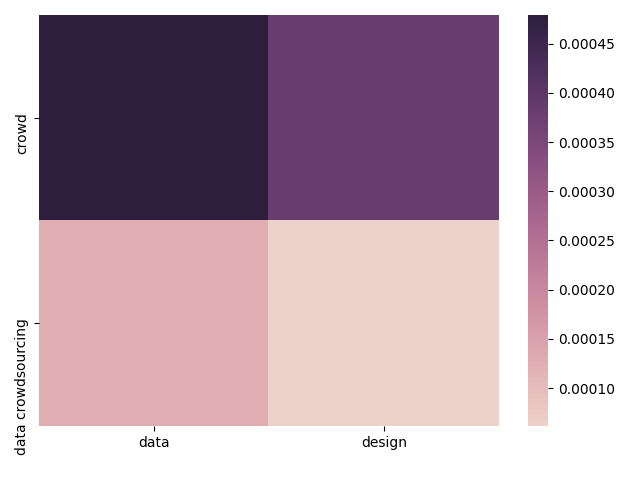
\includegraphics[width=400 pt]{output1.png}
  \caption{Figure 1.}
  \label{fig:matrix}
\end{figure}

Figure \ref{fig:matrix} shows a boat.

\begin{figure}
  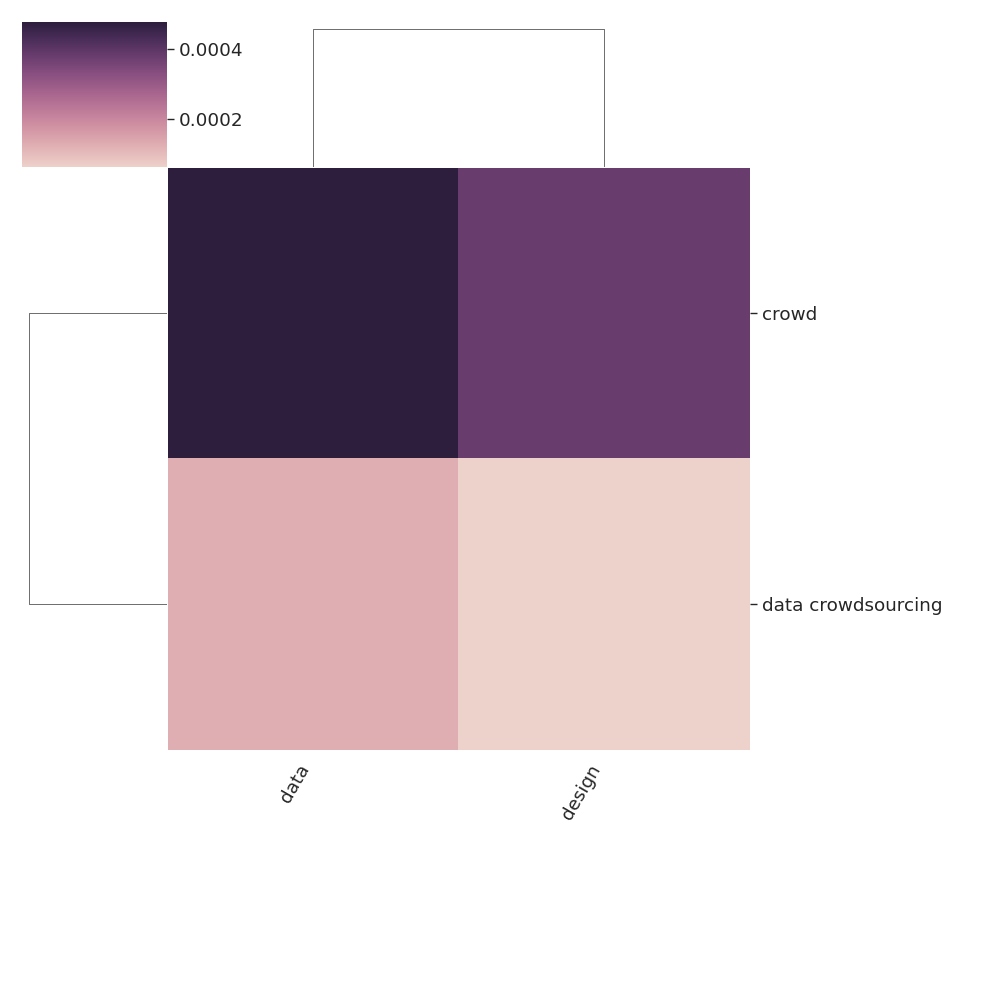
\includegraphics[width=400 pt]{output2.png}
  \caption{Figure 2.}
  \label{fig:2}
\end{figure}

Figure \ref{fig:2} shows a boat.


\VerbatimInput{articles.txt}

\end{document}